\documentclass[11pt,a4paper,oneside]{article}
\usepackage[a4paper,top=2cm,bottom=2.5cm,left=2.5cm,right=2cm]{geometry}
\usepackage[T1]{fontenc}
\usepackage[utf8]{inputenc}
\usepackage[english]{babel}
%\usepackage{frontespizio}
\usepackage{graphicx}
\usepackage{subfig}
\usepackage[english]{varioref}

\begin{document}

%opzione per doppio interlinea
\baselineskip 22pt


%Indice%
\tableofcontents\thispagestyle{empty}\clearpage

\section{Introduction}
\pagenumbering{arabic}
\baselineskip 12pt

\section{The dataset}
The data on which we work are based on the \textbf{CBIS-DDSM} (Curated Breast Imaging Subset of Digital Database for Screening Mammography): it is a set of scanned film mammography studies, adapted to carry out an \textbf{abnormality diagnosis classification}. Following the detailed description attached to each original image, they can be divided into four classes that distinguish whether the represented abnormality patch is a mass or a calcification, and again whether it is benign or malignant. \\
From each original image, the abnormality patch was extracted, and in addition a patch of healthy tissue, adjacent to each abnormality patch, was also extracted. Both abnormality patches and baseline patches have been resized to shape $(150x150)$ and have been added to the final images tensor, that counts 5352 elements (2676 abnormality patches and 2676 baseline patches).
Finally class labels have been assigned to the patches according to the following mapping:
\begin{itemize}
\item 0: Baseline patch
\item 1: Mass, benign
\item 2: Mass, malignant
\item 3: Calcification, benign
\item 4: Calcification, malignant
\end{itemize}

\section{Task 1: Related works}

\clearpage

\section{Task 2: From Scratch CNN}
We developed different models of neural networks to work with the given dataset from scratch and we did different test to find the better hyperparameters to build the final model. This section is divided in three parts: in the first one we describe the main preprocessing applied to the data before the training of the models. Then we show how we built a model for classifying the dataset images between \textit{mass} abnormality and \textit{calfication} abnormality. In the last part, we describe the model built to classify between \textit{benign} and \textit{malignant} abnormality.

\subsection{Data Preprocessing}
Starting from the numpy arrays of the dataset images we were given, first of all we deleted all the samples associated with the \textit{baseline patch} label. Since this labeled images were placed in the even positions of the dataset, we just selected all the odd-index samples al discard the others. This is done both for the training data and the test data. \\
Then we aggregated the labels according to the classification that we needed to do: in the $Task\ 2.1$ the classes \textit{mass benign} and  \textit{mass malignant} were aggregated in a unique class \textit{mass}, and so for the \textit{calcification} classes. On the other hand, in the $Task\ 2.2$ we aggregated  \textit{mass benign} and  \textit{cacification benign} in the \textit{benign} class, and the other labels in the \textit{malignant} class.

\begin{figure}[h]
\centering
	\subfloat[][$Task\ 2.1$: 0 for \textit{mass}, 1 for \textit{calcification} \label{fig:label_mass_calc}]
		{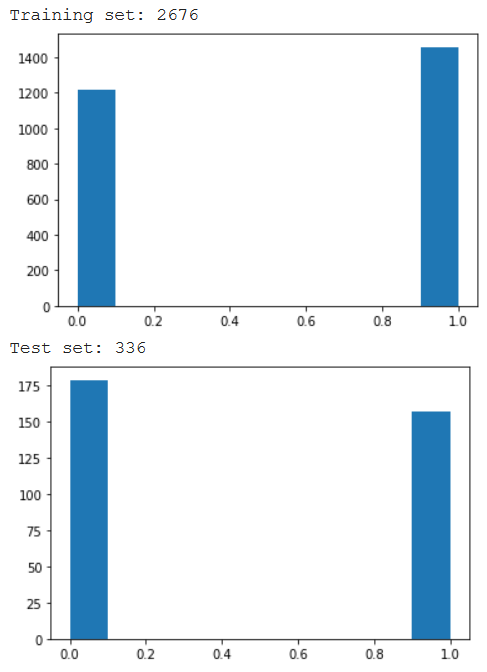
\includegraphics[width=.3\textwidth]{images/label_mass_calc}} \quad
	\subfloat[][$Task\ 2.2$: 0 for \textit{benign}, 1 for \textit{malignant} \label{fig:label_benign_malign}]
		{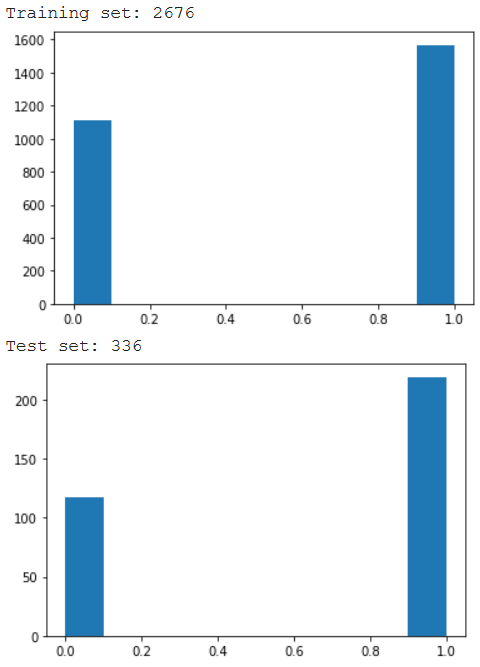
\includegraphics[width=.3\textwidth]{images/label_benign_malign}} \\
\caption{Label distribution}
\label{fig:label distribution}
\end{figure}

For the first case, we can see from the figure that the labels are pretty much equally distributed. Instead, in the second case the dataset is a little more unbalanced towards the \textit{benign} class. \\
Finally, we reshaped all the training images tensors in a single \textit{numpy} array, that has been then normalized. The same has been done for the test images. With regards to the labels, they has been categorizated so that is possible to use the categorical loss function in the model.

\subsection{Task 2.1: Mass-Calcification discriminator}
We first tried to build a simple CNN, with some convolutional and max-pooling layers, and two final dense layers. We trained and tested the model several times, changing the hyperparameters to find a good model for out problem. The final architecture that has been used for the most relevant tests is shown in figure~\ref{fig:scratch_model}. It is made of five convolutional layers, with an increasing number of kernels. Each layer is followed by a max-pooling of $2x2$, except for the last one so that the input of the dense layer is not too reduced. The activation function used in the layers is \textit{ReLu}.

\begin{figure}[h]
\centering
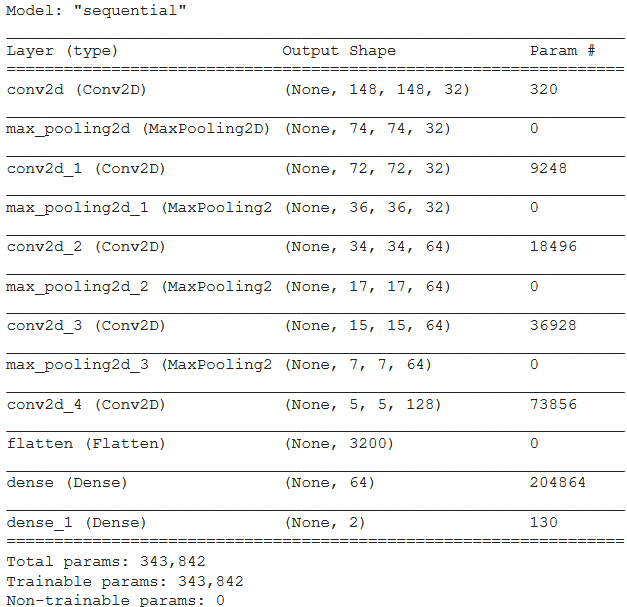
\includegraphics[width=.5\textwidth]{images/scratch_model}
\caption{Architecture of the CNN from scratch ($Task\ 2.1$)}
\label{fig:scratch_model}
\end{figure}

After asserting the architecture, the model has been trained with different numbers of \textit{hidden units} for the first fully connected layer, but also for different \textit{batch sizes} and different \textit{output functions}. 
In all the tests, the conclusion has been that the network was over-training, and this is the reason for which we have developed a second model, adding a data augmentation preprocessing. 
In the figure~\ref{fig:scratch_accuracy}, we present the results in term of accuracy and loss, but also the consufion matrix (fig.~\ref{fig:scratch_matrix}), related to a test of the model with $256$ hidden units, a batch size of $50$, and the \textit{softmax} function for the output layer. 
The used optimizer is Adam, with the deafult learning rate of $0.001$. As we said before, the gap between the training and validation graphs show that the model is over-training: even if the predictions on the test set are accurate, we cannot rely on this network as it is.
\begin{verbatim}
        network.compile(optimizer='adam',
                loss='categorical_crossentropy',
                metrics=['accuracy'])

        network.fit(train_images, train_labels, epochs=100, batch_size=50, 
                validation_split=0.15, shuffle=True, callbacks=[callback])
\end{verbatim}
\begin{figure}[hb]
\centering
	\begin{minipage}[c]{.4\textwidth}
		\centering\setlength{\captionmargin}{0pt}%
		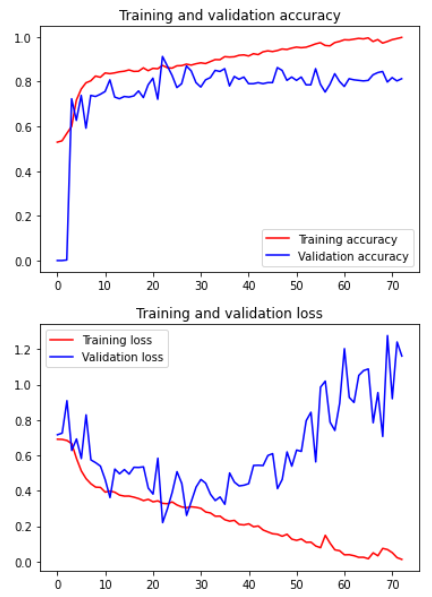
\includegraphics[width=.9\textwidth]{images/scratch_accuracy}
		\caption{Accuracy and loss graphs for the first model training}
		\label{fig:scratch_accuracy}
	\end{minipage}
	\hspace{5mm}%
	\begin{minipage}[c]{.4\textwidth}
		\centering\setlength{\captionmargin}{0pt}%
		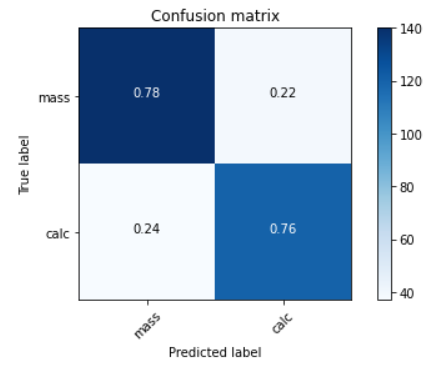
\includegraphics[width=.9\textwidth]{images/scratch_matrix}
		\caption{Confusion matrix for the test-set predictions}
		\label{fig:scratch_matrix}
	\end{minipage}%
\end{figure}

\subsubsection{Data augmentation}
To overcome the problem of over-fitting, we augmented our training using the \textit{ImageDataGenerator} class of \textit{keras}. The main variations we adopted were random rotation up to 40 degrees, random vertical and horizontal shifts with a range of 0.2, random zoom with a range of 0.2, random shear with a range of 0.2 and nearest fill model. To set these parameters we referred to the data in the papers we studied in the initial phase of the project. Before applying these variations to the train set, we splitted it to get the validation set separately.

\begin{verbatim}
        train_set, val_set, train_classes, val_classes = 
                train_test_split( train_images, train_labels, test_size=0.15)
        
        train_datagen = ImageDataGenerator(
                rotation_range=40,
                width_shift_range=0.2,
                height_shift_range=0.2,
                shear_range=20,
                zoom_range=0.2,
                horizontal_flip=True,
                fill_mode='nearest')

        train_generator = train_datagen.flow(train_set,train_classes,batch_size=50)
\end{verbatim}

We trained again our model with the augmented training set and with the validation set, and the results were more satisfying, having a mean accuracy over $80\%$. At this point, we wanted to have a more accurate analysis on some hyperparameters so we did several tests changing their values to get a model as good as possible. 
The tests were regarding the value of the batch size, the number of hidden units, the learning rate and the optimizer itself: we tried using the Adam optimizer and the RMSprop optimizer. Moreover, we also tested the model with different output functions: the softmax and the sigmoid. 
The final accuracy we managed to achieve was $87\%$. This result has been obtained with the Adam optimizer with a learning rate of $0.001$ and with the $softmax$ as the output function for the last FC layer. The batch size was chosen at $50$ and the number of hidden units for the forst FC layer at $256$, both as in the first model without data augmentation. The architecture of the trained network is the same as in figure~\ref{fig:scratch_model}, while the results in terms of accuracy and confusion matrix of the test set are shown in figures~\ref{fig:scratch_accuracy_da} and~\ref{fig:scratch_matrix_da}.
All the tests were done with a maximum of 100 epochs, using the early stopping with a patience of 30.

\begin{figure}[hb]
\centering
	\begin{minipage}[c]{.4\textwidth}
		\centering\setlength{\captionmargin}{0pt}%
		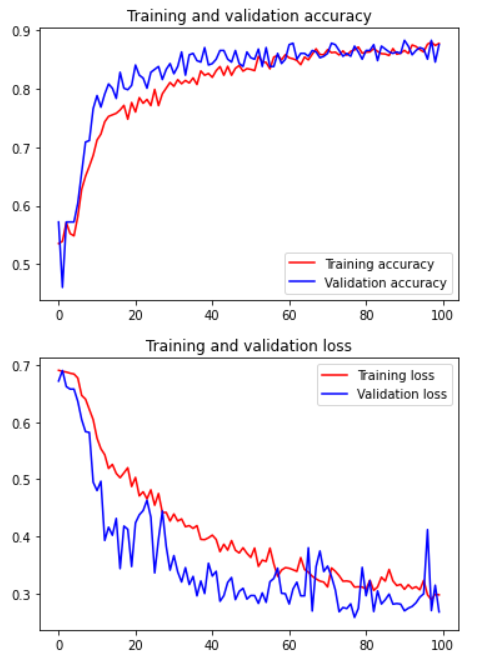
\includegraphics[width=.9\textwidth]{images/scratch_DataAugumentation_2.1/test7/2_adam_acc}
		\caption{Accuracy and loss graphs for the model with data augmentation}
		\label{fig:scratch_accuracy_da}
	\end{minipage}
	\hspace{5mm}%
	\begin{minipage}[c]{.4\textwidth}
		\centering\setlength{\captionmargin}{0pt}%
		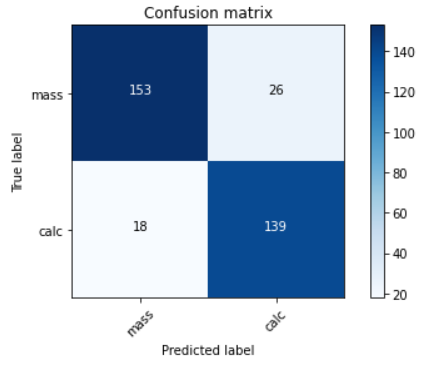
\includegraphics[width=.9\textwidth]{images/scratch_DataAugumentation_2.1/test7/2_adam_matrix}
		\caption{Confusion matrix for the test-set predictions}
		\label{fig:scratch_matrix_da}
	\end{minipage}%
\end{figure}

\clearpage

\subsection{Task 2.2: Benign-Malignant discriminator}
This classification was more complex to accomplish, and the results obtained are not comparable with previous experiments. One of the problems was that the distribution of the two classes was imbalanced in the training set. But the main problem was that distinguishing an abnormality patch between malignant and benign is generally more complex than distinguishing the type of abnormality. 
We spoke with a radiologist and some of his colleagues, and they explained to us that a calcification is very different to a mass: the first is always a very small abnormality, while the second one is almost always bigger. Moreover, they said that mammograms are considered first level examinations, which therefore can leave many doubts about the diagnosis. This is because there are many factors that can limit the visibility and the study of the abnormalities. 
In most cases, abnormalities are best investigated with subsequent examinations, such as ultrasound, MRI, and biopsy.
This complexity remains even in deep learning techniques.\\


As a first approach, we started from the network built in the previous task and we added some modifications, based also on the feedback found on the papers.
We used again the data augmentation, but modifying some of the parameters: in more than one paper it was specified that, to avoid too many distortions in the images, it was necessary to specify a rotation angle multiple of the right angle, and a fill mode of type 'reflect'. Moreover we disabled the horizontal flip of the image, to avoid too much differences from the original set.
We inserted a dropout layer between the two dense layers at the top of the model, with a rate varying from $0.2$ to $0.5$ in the tests.
The better results that we obtained are shown in figures~\ref{fig:accuracy_2.2} and~\ref{fig:matrix_2.2}: the used batch size was still $50$, the hidden units of the first dense layer were $256$, and the learning rate was $0.001$. This model was built with a rate of the dropout layer of $0.2$. 

\begin{figure}[h]
\centering
	\begin{minipage}[c]{.4\textwidth}
		\centering\setlength{\captionmargin}{0pt}%
		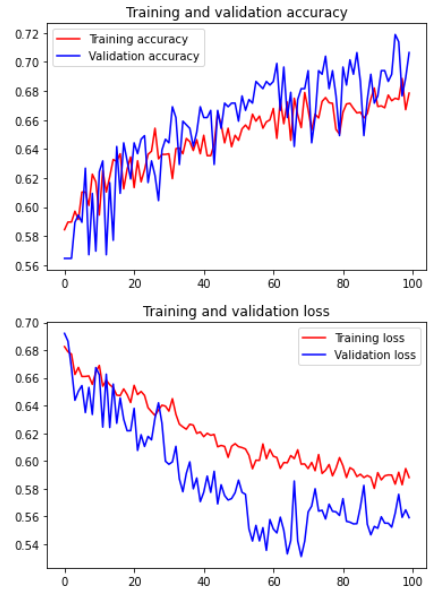
\includegraphics[width=.9\textwidth]{images/2.2/0_acc}
		\caption{Accuracy and loss graphs for the model with data augmentation}
		\label{fig:accuracy_2.2}
	\end{minipage}
	\hspace{5mm}%
	\begin{minipage}[c]{.4\textwidth}
		\centering\setlength{\captionmargin}{0pt}%
		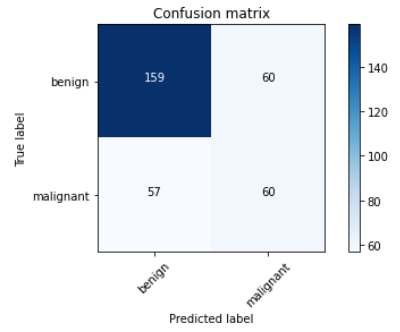
\includegraphics[width=.9\textwidth]{images/2.2/0_matrix}
		\caption{Confusion matrix for the test-set predictions}
		\label{fig:matrix_2.2}
	\end{minipage}%
\end{figure}

As we can see from the graphs, there are some improvement during the training of the network, but very limited. We tried to increment the number of training epochs and the model started to overfitting badly. The major problem is that, predicting the test-set labels, the classifier tended to assign samples to the benign class, when we would have preferred more attention to the malignant class instead, since it is the most critical.\\


We tried to change the architecture of the model again, looking for a structure that could better capture the features of our dataset. After few attempts, we arrived at the model described in figure~\ref{fig:model_2.2_1}, in which we inserted an extra convolutional layer with $128$ kernels, and we decreased the number of hidden units of the FC layer to $128$. This last modification has been done also to simplify the network, decreasing the number of parameters to train in order to reduce the overfitting. The dropout layer remained with a rate of $0.2$.

\begin{figure}[h]
\centering
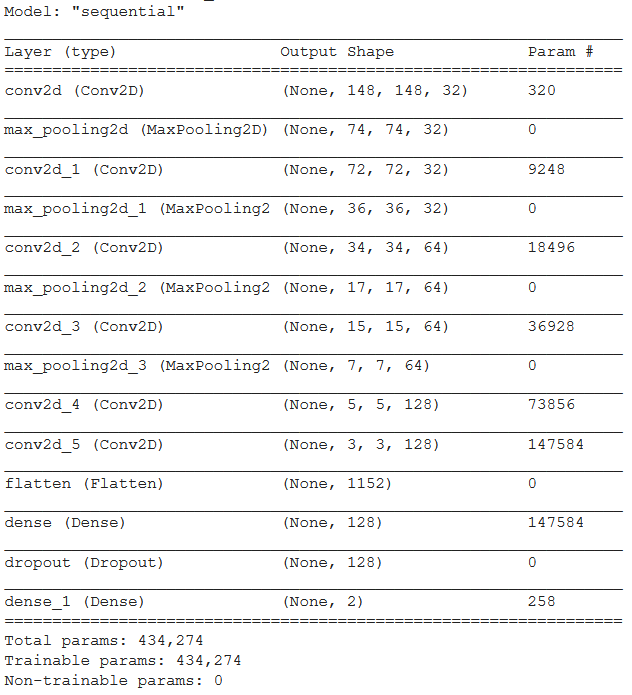
\includegraphics[width=.5\textwidth]{images/2.2/1_model}
\caption{Architecture of the CNN from scratch ($Task\ 2.2$)}
\label{fig:model_2.2_1}
\end{figure}

The results (fig.~\ref{fig:accuracy_2.2_1} and~\ref{fig:matrix_2.2_1}) in terms of accuracy and loss were very similar to the previous model, but we can see from the confusion matrix that the \textit{malignant} class was better predicted and we considered it as a good result.

\begin{figure}[h]
\centering
	\begin{minipage}[c]{.4\textwidth}
		\centering\setlength{\captionmargin}{0pt}%
		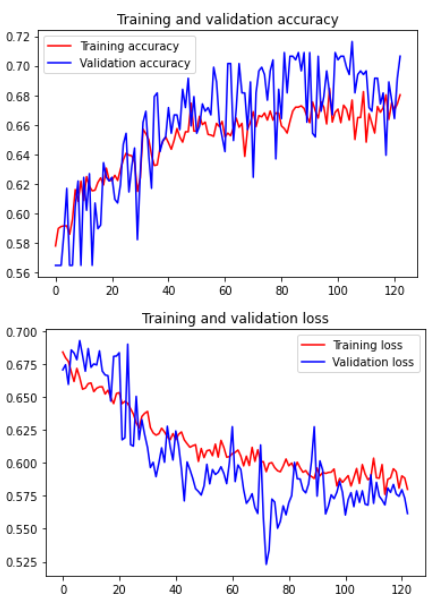
\includegraphics[width=.9\textwidth]{images/2.2/5_acc}
		\caption{Accuracy and loss graphs for the model with data augmentation}
		\label{fig:accuracy_2.2_1}
	\end{minipage}
	\hspace{5mm}%
	\begin{minipage}[c]{.4\textwidth}
		\centering\setlength{\captionmargin}{0pt}%
		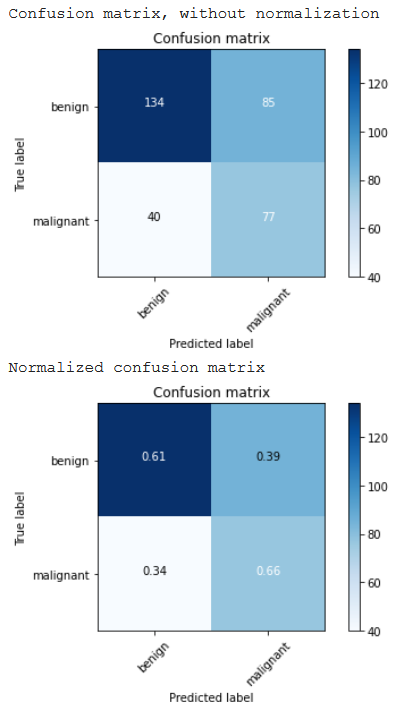
\includegraphics[width=.9\textwidth]{images/2.2/5_matrix}
		\caption{Confusion matrix for the test-set predictions}
		\label{fig:matrix_2.2_1}
	\end{minipage}%
\end{figure}

Trying to solve the unbalancing of the two classes, we assigned weights to them so that their unbalance in the training set would be considered. We have trained again the network, passing the new weights of the classes as parameters: the results are found in the figures~\ref{fig:accuracy_2.2_1_weights} and~\ref{fig:matrix_2.2_1_weights}. 

\begin{verbatim}
    weight_for_benign = (1 / benign)*(total)/2.0 
    weight_for_malignant = (1 / malignant)*(total)/2.0
    
    > Total samples: 2274
    > Benign samples: 1341
    > Malignant samples: 933
    > Weight for benign: 0.85
    > Weight for malignant: 1.22
\end{verbatim}

\begin{figure}[h]
\centering
	\begin{minipage}[c]{.4\textwidth}
		\centering\setlength{\captionmargin}{0pt}%
		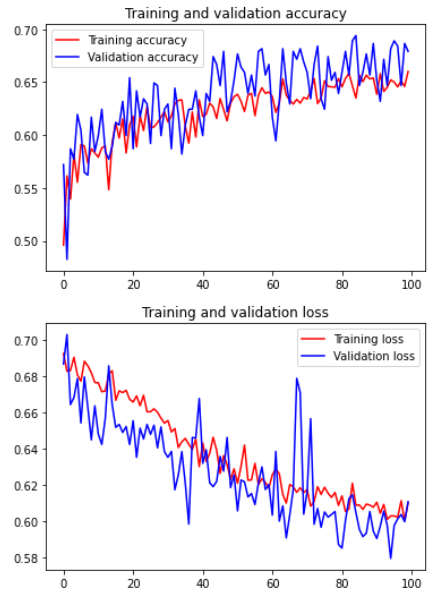
\includegraphics[width=.9\textwidth]{images/2.2/7_acc}
		\caption{Accuracy and loss graphs for the model with data augmentation}
		\label{fig:accuracy_2.2_1_weights}
	\end{minipage}
	\hspace{5mm}%
	\begin{minipage}[c]{.4\textwidth}
		\centering\setlength{\captionmargin}{0pt}%
		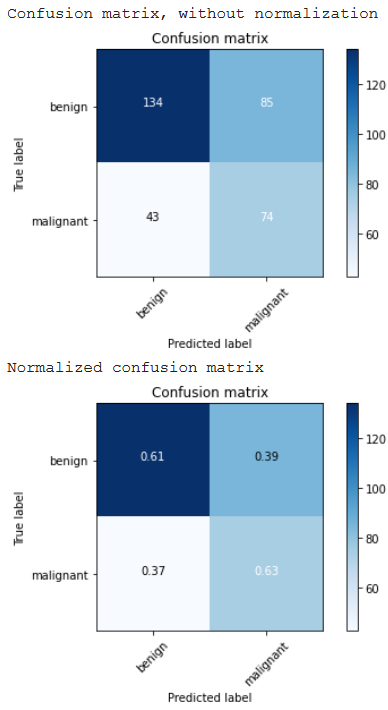
\includegraphics[width=.9\textwidth]{images/2.2/7_matrix}
		\caption{Confusion matrix for the test-set predictions}
		\label{fig:matrix_2.2_1_weights}
	\end{minipage}%
\end{figure}



Finally, we tried a different approach to see if performance could improve. We used the data augmentation functions to create a new training set with a larger number of samples: from each image we created four more, applying the \textit{ImageDataGenerator} transformations, and obtaining a new dataset of $13.380$ samples.

\begin{verbatim}
    from keras.preprocessing.image import ImageDataGenerator
    variations_per_img = 4
    train_datagen = ImageDataGenerator(
        rotation_range=90,
        width_shift_range=0.2,
        height_shift_range=0.2,
        shear_range=20,
        zoom_range=0.2,
        fill_mode='reflect')

    for i in range(0,len(train_images)):
      new_train_images.append(train_images[i])
      new_train_labels.append(train_labels[i])
  
      train_generator = train_datagen.flow(
  	    	train_images[i].reshape(1,150,150,1),batch_size=1)
      for j in range(variations_per_img):
        new_train_images.append(train_generator.next().reshape(150,150))
        new_train_labels.append(train_labels[i])
      del train_generator
\end{verbatim}

The classification did not improve, and indeed this model was experimenting a higher rate of over-fitting. We tried again to reduce the over-training, by adding some dropout layers, also between the convolutional layers, by further simplifying the model, and by decreasing the learning rate, but we did not succeeded.

\subsubsection{Mass benign - mass malignant discriminator}


\section{Task 3: Pretrained network}

\subsection{Task 3.1: Mass-Calcification discriminator}


\subsubsection{ VGG16 }

\subsection{Task 3.2: Benign-Malignant discriminator}


\section{Task 4: Baseline patches}


\section{Task 5: Ensemble network}

\end{document}
